\documentclass[a4paper, 12pt]{article}
\usepackage{fullpage}
\usepackage[utf8]{inputenc}
\usepackage[english]{babel}
\usepackage{latexsym}
\usepackage{color}
\usepackage{amssymb}
\usepackage{amsmath}
\usepackage{graphicx}
\usepackage{fancyhdr}
\usepackage{caption}
\usepackage{subfigure}


\pagestyle{fancy}
\fancyhf{}
\fancyhead[RE,LO]{Project 2: Learning of Grid Cells}
\headsep=15mm

\title{Project 2: Learning of Grid Cells}
\author{Claus Lang, Can Eren Sezener, Claudia Winklmayr}
\date{09.02.2016}


\begin{document}
\maketitle

\paragraph{Abstract:}
Grid cells, located in rats medial entorhinal cortex (mEC), show increased firing activity when the animal enters specific regions of the environment and their firing maps show a characteristic hexagonal grid pattern. In our project we implement a computational model for the development of grid cells that was first introduced by Kropff and Treves in 2008 ([1],[2]). We simulate a rat exploring a square environment at constant speed and model the development of grid cell activity in a population of neurons receiving spacially tuned feed forward imput. 
 

\section{Introduction}
Different types of neurons encode the spatial location of an animal. Place cells - located in hippocampus - were discovered in the 1970s by O'Keefe and Dostrovsky [3], they show increased activity when the animal enters a specific region of the environment - the so-called place field.\newline
Grid cells - located in medial entorhinal cortex (mEC) were then discovered in 2005 [4]. In contrast to place cells, grid cells are activated at multiple locations and their firing maps show a characteristic hexagonal grid pattern. Grid cells can be characterized by spacing, orientation and spatial phase. Neighbouring grid cells show similar spacing and orientation. \newline
It was proposed that grid cells perform a path integration task, taking into account the rat's current position, its running speed and direction of movement. Sensual information, on the other hand, was attributed a secondary role in the formation of the grid patterns [5]. \newline
%
%
%
\section{Model}
The Kropff and Treves model assumes places cells as the basis for grid cell development. In our implementation the model consists of a layer of 400 input neurons (simulating place cells) and 100 output neurons (simulation grid cells). Every unit of the input layer is connected to every unit of the output layer. This is schematically visulaized in figure \ref{overview}. At each time step the place cells receive spatially tuned input encoding the rat's current position. Every output unit then receives input from all place cells and the weights connecting input and output neurons are updated by a Hebbian learning rule. 

\begin{center}
\begin{figure}\label{overview}
\begin{center}
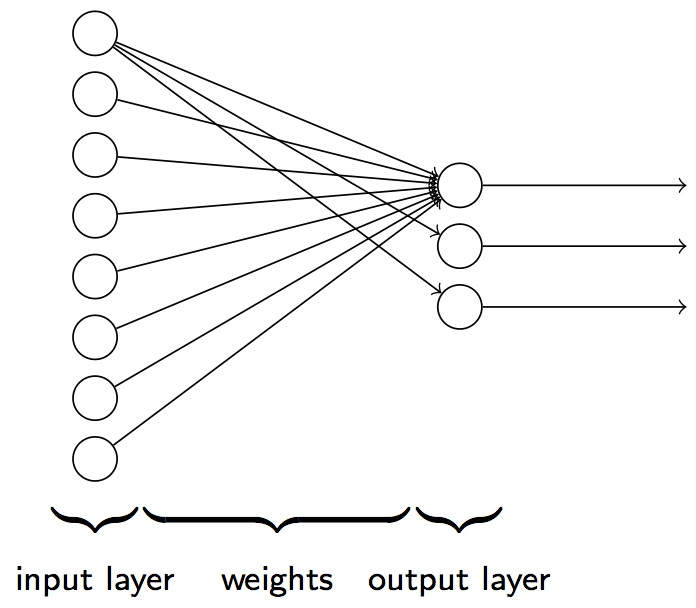
\includegraphics[width=0.6\textwidth]{pics/model_overview.png}
\footnotesize{\caption{The feed-forward network (showing only a subset of the nodes and only all connections from one input node and to one output node)}}
\end{center}
\end{figure}
\end{center}

\subsection{Spatial exploration}
\begin{figure}[h]
\begin{minipage}{0.4\textwidth}
	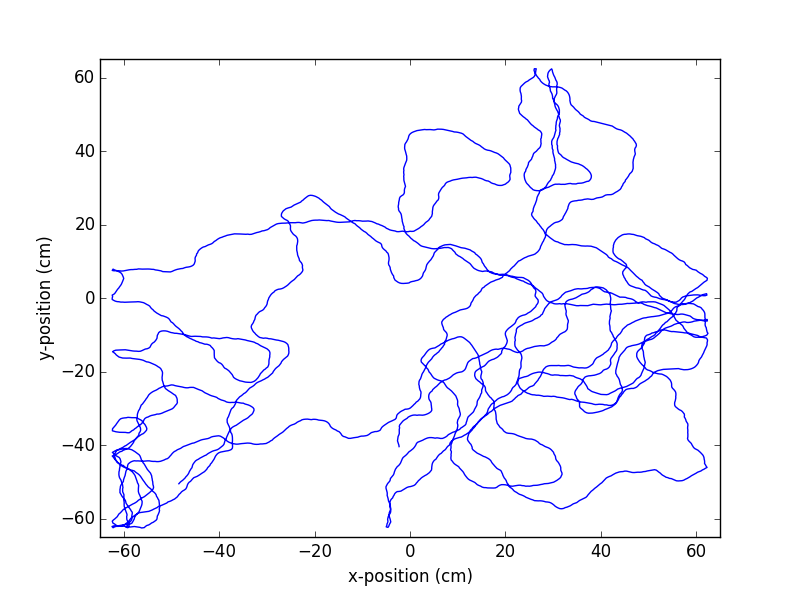
\includegraphics[width=6cm, height=6cm]{pics/running_rat.png}
	\footnotesize{\caption{trajectory of the virtual rat exploring for 50 seconds}}
\end{minipage}
\begin{minipage}{0.6\textwidth}
To create the spatial coordinates that serve as input for the first layer of neurons, we simulate a rat exploring a square environment of size 125 cm $\times$ 125 cm at a speed of 0.4 m/s. At each time step $\tau=$10 ms we chose a new direction by randomly drawing an angle $\phi$ from a normal distribution, which is centred around the direction at the previous time step and has a standard deviation of 0.2 rad.   
\end{minipage}
\end{figure}

\subsection{Input layer}
The input layer consists of 400 place units processing information about the rats location $\boldsymbol{x}(t)$ at a given time $t$ (see figure \ref{input}). The firing $r_j^{in}(t)$ of each place unit is modelled by a Gaussian function centred around the cell's preferred location $\boldsymbol{x}_j$. The width of the firing field is denoted by $\sigma_p=$ 5 cm. 
	\begin{equation}
	r_j^{in}(t)=\exp\left(\frac{-|\boldsymbol{x}^t-\boldsymbol{x}_j|}{2\sigma_p^2}\right)
	\end{equation}
In figure 2 we can see the activation of input layer neurons as the rat explores a small section of the environment:  

\begin{figure}[h]\label{input}
\setlength{\abovecaptionskip}{5pt}
\setlength{\belowcaptionskip}{0pt}
\begin{minipage}[t]{0.3\textwidth}\vspace{0pt}
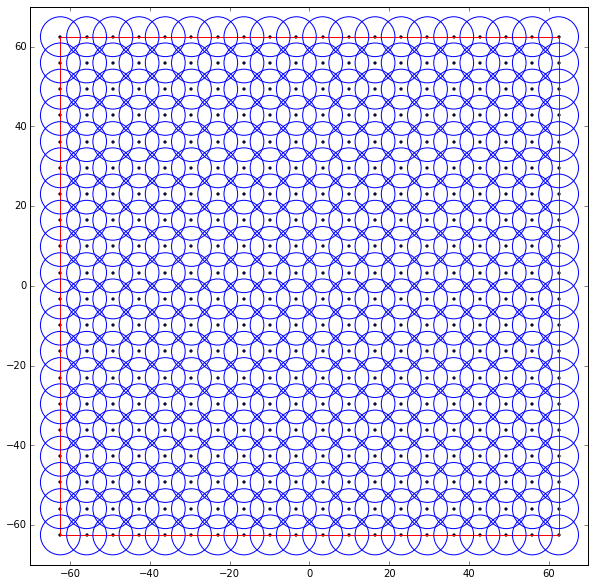
\includegraphics[width=4cm, height=4cm]{pics/place_cell_locations}
\end{minipage}\hfill%
\begin{minipage}[t]{0.3\textwidth}\vspace{0pt}
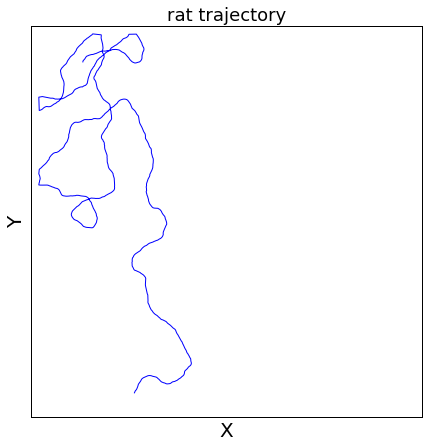
\includegraphics[width=4cm, height=4cm]{pics/mouse_demo}
\end{minipage}\hfill
\begin{minipage}[t]{0.3\textwidth}\vspace{0pt}
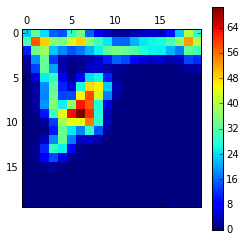
\includegraphics[width=5cm, height=5cm]{pics/activity_demo}
\end{minipage}
\caption{\footnotesize{From left to right: (i) Distribution of place fields across the environment, (ii) Trajectory of the virtual rat and (iii) Activity of place cells summed over exploring time. Each pixel corresponds to one place cell (arranged as in (i)).}}
\end{figure}
%
%
%	
\subsection{Output layer}
At each time step output unit $i$ receives as input a weighted sum $h_i$ of the place cell activities: 
	\begin{equation}
	h_i(t)=\sum_jw_{ij}r_j^{in}(t).
	\end{equation}
By $w_{ij}$ we denote the weight of the connection from the $j$-th input unit to the $i$-th output unit. $h_i(t)$ is then subject to an dynamic adaptation process involving the activation variable $r^+$ and the inactivation variable $r^-$. The speed of the adaptation is governed by the time constants $\tau^+=0.1$ s and $\tau^-=0.3$ s:
	\begin{eqnarray}
	\tau^+\frac{d}{dt}r^+_i &=& h_i(t)-r^+_i(t)-r^-_i(t)\\
	\tau^-\frac{d}{dt}r^-_i &=& h_i(t)-r^-_i(t)
	\end{eqnarray}
In order to understand the dynamics of this system of differential equations, consider a sinusoidal input of $h_i(t) = \sin(\pi k t^2)$. Figure \ref{adaptation} shows the numerical solution of $r^+_i$ in that case plottet versus the frequency of the input $kt$. The plot shows that there is a resonance frequency of about $0.92 \frac{1}{s}$, where the activation $r^+_i$ is maximal.
\begin{figure}[h]
	\begin{center}
	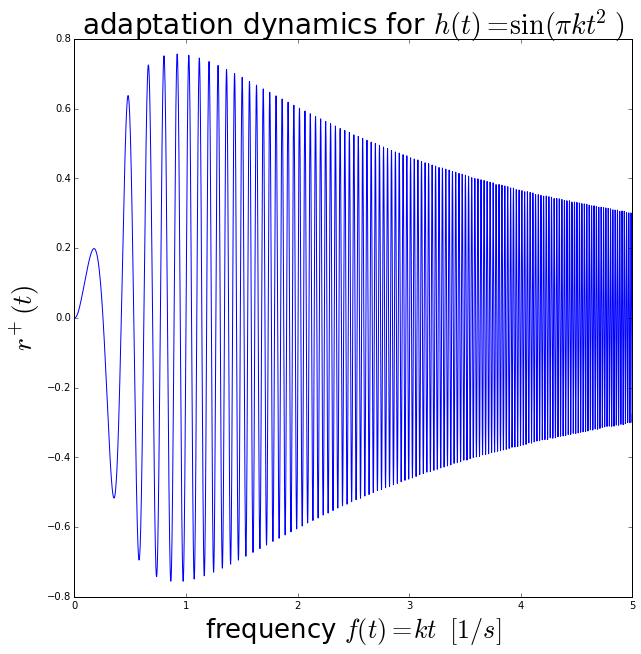
\includegraphics[width=6cm, height=6cm]{pics/sinusoidal_activation}
	\footnotesize{\caption{numerical solution of adaptation dynamics for sinusoidal input}}
	\end{center}
\end{figure}

\noindent The variable $r^+$ is then used to calculate the final output via the following activation function: 
	\begin{equation}
	r_i^{out}(t)=\frac{2}{\pi}\arctan(g(r_i^+(t)-\mu))\Theta( r_i^+(t)-\mu).
	\end{equation}
The Heaviside step-function $\Theta$ ensures that all output values are nonnegative and the factor $\frac{2}{\pi}$ serves to normalize them to values between 0 and 1.  \newline
The two control parameters $g$ and $\mu$ are the gain and the threshold of the system. $g$ serves to keep the mean activity across neurons - defined via $a= \frac{1}{N}\sum_ir_i^{out}$- within a 10\%-range from the value $a_0$. The parameter $\mu$ respectively controls the sparsity $s=\frac{(\sum_ir_i^{out})^2}{\frac{1}{N}\sum_i (r_i^{out})^2}$ and keeps it within a 10\% error bound of the value $s_0$. In both above expressions the parameter $N$ denotes the number of output neurons. We determine $g$ and $\mu$ by an optimization algorithm where at each step they are updated in the following way: 
	\begin{eqnarray}
	\mu^{t, l+1} &=& \mu^{t,l}+b_\mu(a^{l}-a_0)\\
	g^{t,l+1} &=& g^{t,l}+ b_gg^{t,l}(s^l-s_0)
	\end{eqnarray}
\noindent $l$ indicates the step of the iteration. The updating process is stopped if both $a$ and $s$ fall within the 10 \% error bound of $a_0$ and $s_0$ or when an upper bound of 100 iterations is reached. 
	
\begin{figure}[h]
\setlength{\abovecaptionskip}{5pt}
\setlength{\belowcaptionskip}{0pt}	
	\begin{minipage}[t]{0.5\textwidth}\vspace{0pt}
	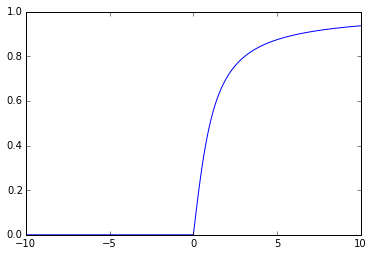
\includegraphics[width=5cm, height=4cm]{pics/output_function.png}
	\footnotesize{\caption{Activation function for\\ output neurons}}
	\end{minipage}
\hfill
	\begin{minipage}[t]{0.5\textwidth}\vspace{20pt}
	\begin{tabular}{c|cccccc}
	& $a_0$ & $s_0$ & $\mu^{0,0}$ & $g^{0,0}$ & $b_\mu$ & $b_g$\\
	\hline\\
	& 0.1 & 0.3 & 0 & 4.5 & 0.01 & 0.1\\
	\end{tabular}
	\footnotesize{\captionof{table}{Default parameters for adaptation dynamics}}
	\end{minipage}
\end{figure}	
%
%
%
\subsection{Weights}
The weights between the input and the output layer are initially being drawn from a uniform distribution in $[0,1]$ and normalized to unit norm i.e. for every output unit $i$ we impose $\sum_jw^2_{ij}=1$. At each timestep of the simulation the weights are then updated using a Hebbian learning rule:  
\begin{equation}
w_{ij}(t+\Delta t)= w_{ij}(t)+ \epsilon(r_i^{out}(t)r_j^{in}(t)-\overline{r}_i^{out}(t)\overline{r}_j^{in}(t)),
\end{equation}
$\epsilon= 0.005$ is a moderate learning rate and $\overline{r}_i^{out}(t)$ and $\overline{r}_j^{in}(t)$ are the running averages of input and output firing rates.  
	\begin{eqnarray}
	\overline{r}_i^{out}(t) &=& \overline{r}_i^{out}(t-1)+ \eta(r_i^{out}(t)-\overline{r}_i^{out}(t-1))\\
	\overline{r}_j^{in}(t) &=& \overline{r}_j^{in}(t-1)+ \eta(r_j^{in}(t)-\overline{r}_j^{in}(t-1)).
	\end{eqnarray}
$\eta=0.05$ sets the time averaging constant. After each update the weights are kept normalized to unit norm. 
%
%
\section{Results}
We ran the simulation for 2.5 hours in rat time. The results show that this duration is sufficient for grid cells to develop. Figure \ref{time-evol} shows the time evolution of weights of a grid cell. The cell we picked has one of the most apparent grid structure among the other cells.

%\subsection{Time evolution}
\begin{figure}[htbp]
\begin{minipage}[hbt]{0,49\textwidth}
        \centering
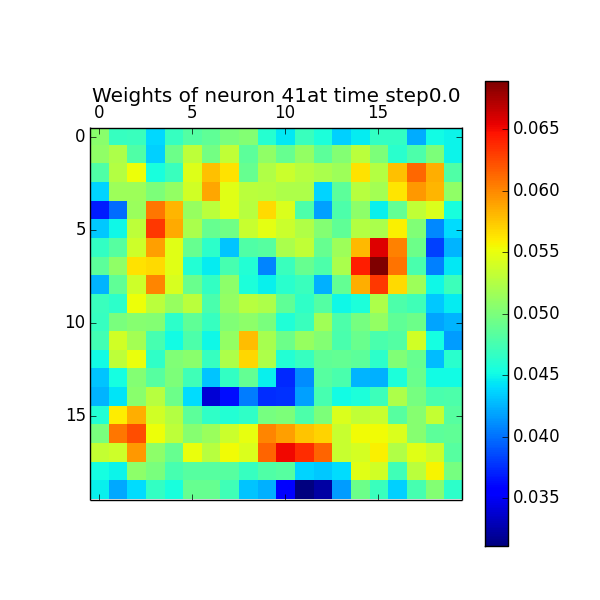
\includegraphics[width=6cm,height=6cm]{neurons/neuron_w_41_t_0.png}\\[10pt]
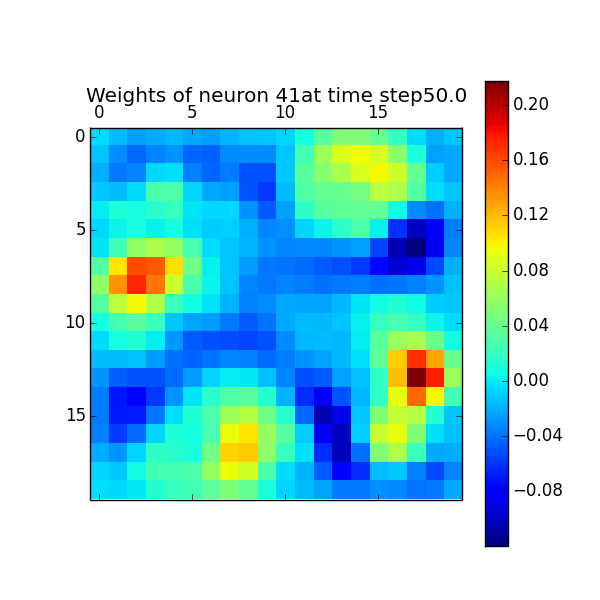
\includegraphics[width=6cm,height=6cm]{neurons/neuron_w_41_t_50.png} \\[10pt]
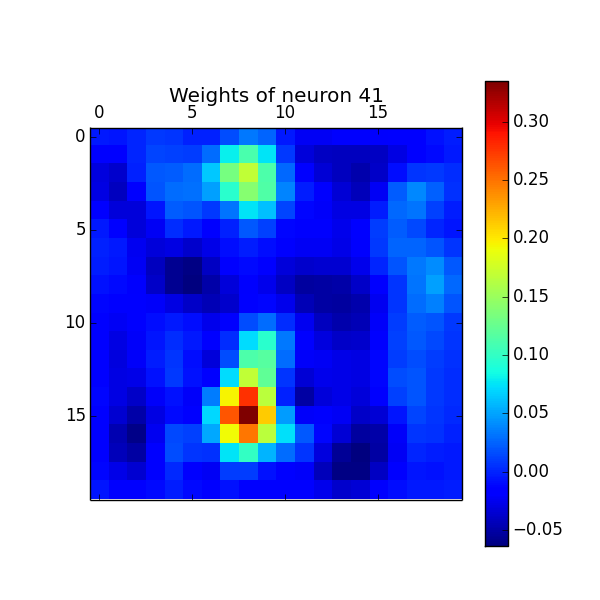
\includegraphics[width=6cm,height=6cm]{neurons/neuron_w_41.png}
        \caption{weight development}
        \label{LabelA}
\end{minipage}
\begin{minipage}[hbt]{0,49\textwidth}
        \centering
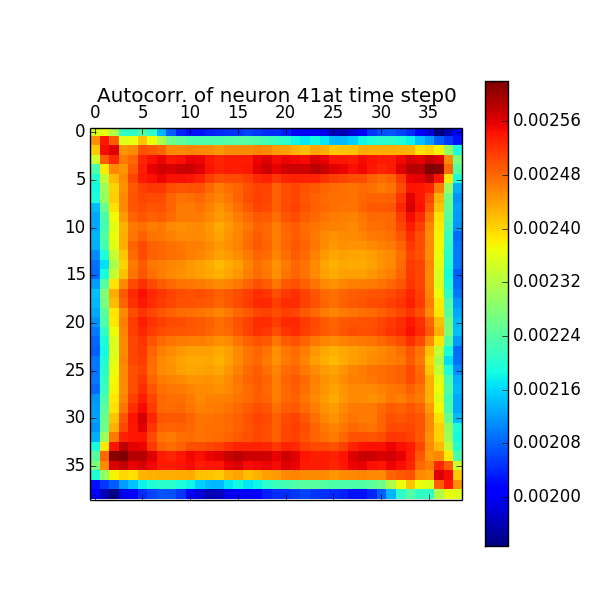
\includegraphics[width=6cm,height=6cm]{neurons/neuron_a_41_t_0.png}\\[10pt]
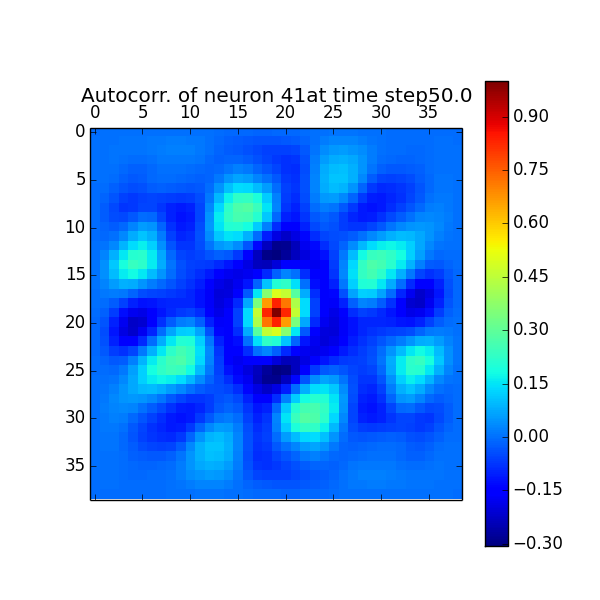
\includegraphics[width=6cm,height=6cm]{neurons/neuron_a_41_t_50.png}\\[10pt]
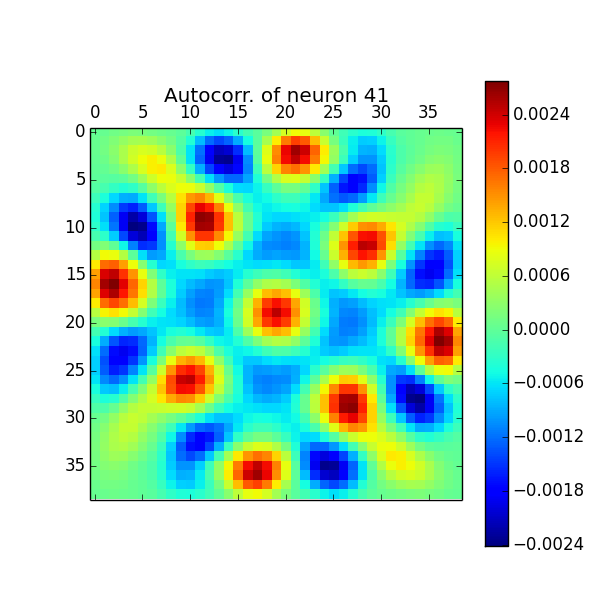
\includegraphics[width=6cm,height=6cm]{neurons/neuron_a_41.png}
        \caption{autocorrellation development}
        \label{LabelB}
\end{minipage}
\centering
\caption{The weights and the autocorrelogram of a neuron at the beginning, middle and the end of the simulation}
\label{time-evol}
\end{figure}

When all grid cells are inspected, it is seen that most grid cells have similar spatial frequencies, however, their orientations and off-sets are different. Figure \ref{diff} illustrates this difference. 

\begin{figure}
\hfill
\subfigure{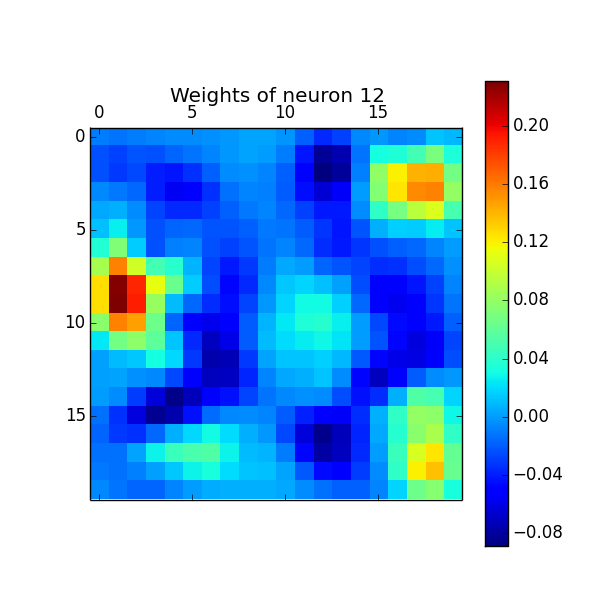
\includegraphics[width=6cm]{neurons/neuron_w_12.png}}
\hfill
\subfigure{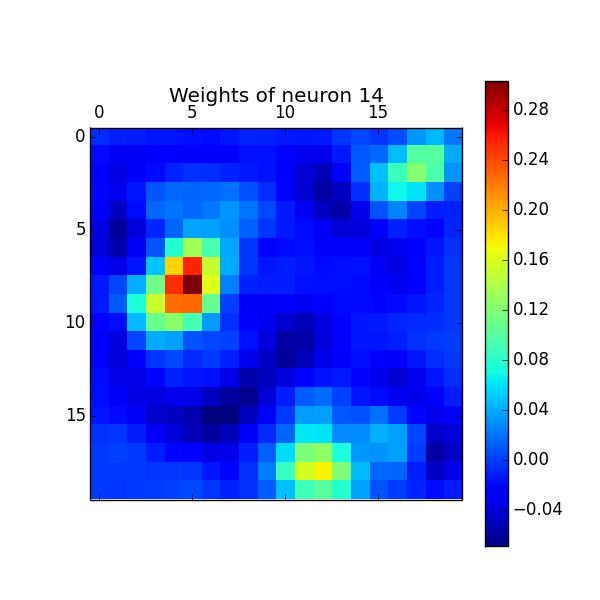
\includegraphics[width=6cm]{neurons/neuron_w_14.png}}
\hfill
\caption{Different grid cells have different orientations and off-sets but similar spatial frequencies.}
\label{diff}
\end{figure}
%
%
%

\newpage
\section{References}
\begin{enumerate}
\item E.Kropff and A.Treves, \textit{The Emergence of Grid Cells: Intelligent Design or Just Adaptation?}, Hippocampus 18: 1256-1269 (2008).

\item B. Si, E. Kropff, and A. Treves, \textit{Grid alignment in entorhinal cortex.} Biological cybernetics 106: 8-9 (2012).

\item J. O'Keefe and J.Dostrovsky,\textit{The hippocampus as a spatial map. Preliminary evidence from unit activity in the freely-moving rat.} Brain Res. 34:171-175 (1971). 

\item T. Hafting, M. Fyhn, S. Molden, M.-B. Moser and E.I.Moser,\textit{Microstructure of a spatial map in the entorhinal cortex.} Nature 436: 801-806 (2005).

\item J.S.Barlow,\textit{Inertial navigation as a basis for animal navigation.} J Theor Biol. 6:  76-117 (1964)
\end{enumerate}


\end{document}

	